\chapter{Introduction}

\section{Motivation}
Scaling of CMOS technology has progressed significantly, defying barriers in manufacturing processes. It has benefited us mainly in terms of significant performance improvements and reduced dimensions of the final product. However the reduction in the supply voltages and increase in operating frequencies, which have also accompanied scaling, have resulted in higher error rates \cite{Srinivasan2004, Constantinescu2007, Agostinelli2005}.

Errors that occur on semiconductor chips  can be attributed to permanent, transient or intermittent faults. Permanent faults are caused primarily by irreversible changes, like an open or a short link. Transient faults are caused by temporary environment conditions, e.g. cosmic rays. Intermittent faults are caused by an unstable or marginal state of the hardware \cite{Constantinescu2007}. Intermittent failures can go away with time or may manifest later into a permanent breakdown, depending on underlying defect mechanism. Only way to correct failures caused by permanent faults is to replace the offending component.  Transient faults occur rarely in the device lifetime, and manifest themselves as soft errors. Some of these failures, specially  failures due to transient faults can be avoided by using fault tolerance mechanisms \cite{Bartlett2004, Mitra2008}. While the fault tolerance circuits can significantly reduce failure rates, these circuits themselves can be affected by one of the faults.

In safety critical systems all of the faults should be treated equally and circuits which have any of these faults should be rejected. However, a large portion of semiconductor applications are not safety critical. For those applications, permanent faults and the those intermittent faults which can severely degrade functionally, can be assumed as \emph{critical}, while all other types of faults can be assumed to be \emph{non-critical}

During post-production testing of these chips, they are categorized as either faulty or working \cite{Agrawal2000}. No further attempt is made to check if circuits had any non-critical faults. This approach leads to yield loss, as some of the healthy chips which had only transient faults are also rejected. An alternative approach that can be explored is shown in figure~\ref{fig:proposedflow}. It is proposed that if the chips can be separated as working and partially working, the partially working ones can still be included in the final yield of the product, without degradation of the quality and still reducing yield loss.

\begin{figure}[h]
  \begin{center}
    \captionsetup{justification=centering}
    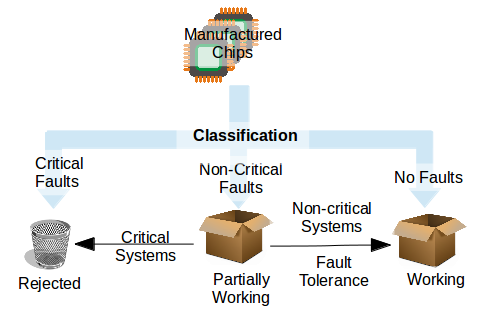
\includegraphics[scale=0.55]{figures/proposedflow.png}
    \caption{Proposed classification flow for VLSI Chips}
    \label{fig:proposedflow}
  \end{center}
\end{figure}

With scaling is expected that, non-critical failures (\emph{i.e.} failures due to transient faults) will constitute majority of failures \cite{Constantinescu2003}. Hence a significant yield loss can be avoided by using the method proposed above. This can be achieved if we are able to classify faults as permanent, transient and intermittent, then reject circuits with permanent and intermittent faults, while retaining chips transient faults. Such classification can also help designers with statistics about failures, which can be useful to find underlying defect mechanism, resulting in further improvement of the product quality.

Classification of faults into such categories is difficult as intermittent faults and transient faults manifest similarly. This is even more apparent, as systems move to lower technology nodes. It then becomes difficult to classify faults with traditional approaches, as criteria used for classification are not conclusive. This ambiguity, and the fact that problem at hand is changing as technology continues to evolve, calls for an alternative approach, which is adaptive and where the system can classify faults accurately.

Machine learning techniques are shown to be useful in cases, where it is difficult to express knowledge in terms of fixed set of rules. Machine learning approaches have shown that the the lack of knowledge can be covered up with data \cite{Alpaydin2004}. In our case, the ambiguity of the classification rules can be covered up by storing past classification decisions and \enquote{learn} from those for accurate classification. The primary focus of the thesis is to explore the possibility of fault classification by using machine learning approach.

\section{Thesis Organization}
This thesis report is organized as follows:
\begin{description}
\item[Chapter~\ref{chap:chapter2} -- \nameref{chap:chapter2}:] The first part of this chapter defines the fault taxonomy used for classification. It covers the definition, sources and fault models used for each of the fault types. It also notes characteristics for fault types used to derive feature in later chapters. Second part of the chapter covers related work done to classify faults in computing systems and on VLSI chips. Third part presents a brief account of fault diagnosis and diagnostic parameters.

\item[Chapter~\ref{chap:chapter3} -- \nameref{chap:chapter3}:] This chapter covers some basic terms and definitions used in machine learning. It explains supervised and unsupervised approaches in machine learning. A brief survey of some of the popular machine learning algorithms are covered in this chapter, along with their training procedures and advantages and disadvantages of while using each of them for classification.
 
\item[Chapter~\ref{chap:chapter4} -- \nameref{chap:chapter4}:] A detailed account of the problem definition is covered in the first part of this chapter. Second part covers feature selection for classification and their extraction methods.

\item[Chapter~\ref{chap:chapter5} -- \nameref{chap:chapter5}:] This chapter starts with assumptions and experimental setup to generate sample population and test data for learning is explained in this chapter. Rest of the chapter focuses on procedure to train the classifier and using the same for fault classification.

\item[Chapter~\ref{chap:chapter6} -- \nameref{chap:chapter6}:] Results obtained using the techniques described in chapter~\ref{chap:chapter4} and~\ref{chap:chapter6} are presented in this chapter.

\item[Chapter~\ref{chap:chapter7} -- \nameref{chap:chapter7}:] This chapter concludes the thesis and summarizes possible applications of method suggested in this thesis and the future work.
\end{description}
